\documentclass[numbers]{article}
\usepackage{amsmath,amsfonts}
\usepackage{xcolor}
\usepackage{tikz}
\usepackage{pgfplots}
\usetikzlibrary{positioning,arrows}
\usepgfplotslibrary{colorbrewer}
\pgfplotsset{
  xlabel near ticks,
  ylabel near ticks,
}

\begin{document}

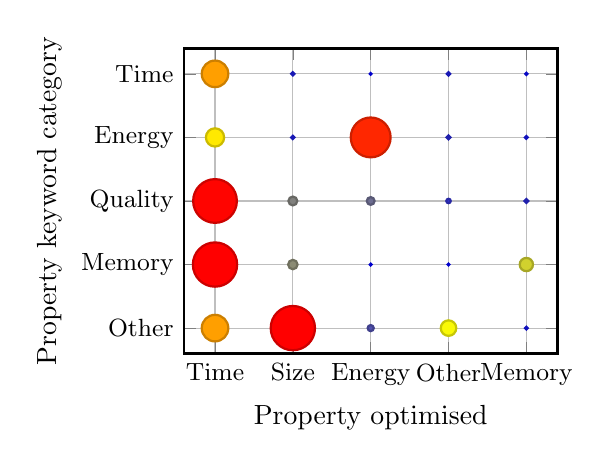
\begin{tikzpicture}
    \begin{axis}[
        width=18em,
        xlabel={Property optimised},
        ylabel={Property keyword category},
        xtick=data,
        ytick=data,
        symbolic x coords={Time,Size,Energy,Other,Memory},
        symbolic y coords={{Other},{Memory},{Quality},{Energy},{Time}},
        grid,
        thick,
        cycle list/Set1,
        every tick label/.append style={font=\small},
      ]
      \addplot[%
          scatter=true,
          only marks,
          mark=*,
          point meta=explicit,
          visualization depends on = {0.10*\thisrow{v} \as \perpointmarksize},
          scatter/@pre marker code/.append style={/tikz/mark size=\perpointmarksize},
      ] table [x=x,y=y,meta index=2,col sep=semicolon,trim cells] {
x ; y ; v
Time ; {Other} ; 48.000000
Size ; {Other} ; 80.000000
Energy ; {Other} ; 11.000000
Other ; {Other} ; 28.000000
Memory ; {Other} ; 5.000000
Time ; {Memory} ; 80.000000
Size ; {Memory} ; 17.000000
Energy ; {Memory} ; 3.000000
Other ; {Memory} ; 3.000000
Memory ; {Memory} ; 24.000000
Time ; {Quality} ; 79.000000
Size ; {Quality} ; 16.000000
Energy ; {Quality} ; 14.000000
Other ; {Quality} ; 8.000000
Memory ; {Quality} ; 7.000000
Time ; {Energy} ; 33.000000
Size ; {Energy} ; 6.000000
Energy ; {Energy} ; 72.000000
Other ; {Energy} ; 7.000000
Memory ; {Energy} ; 5.000000
Time ; {Time} ; 48.000000
Size ; {Time} ; 6.000000
Energy ; {Time} ; 3.000000
Other ; {Time} ; 6.000000
Memory ; {Time} ; 4.000000
};
    \end{axis}
  \end{tikzpicture}

\end{document}